\subsection{$\mathrm{BP}$ 神经网络训练与检验}

  \subsubsection{神经网络训练}
    \begin{figure}[htbp]
      \centering
      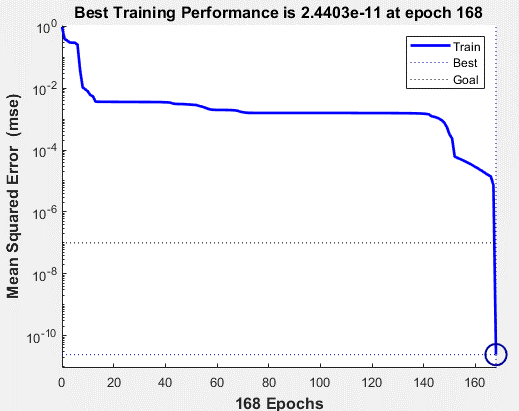
\includegraphics[width=0.618\paperwidth]{figures/muxinxunlian.png}
      \caption{神经网络训练}
      \label{fig:wanluoxunlian}
    \end{figure}
    由图 \ref{fig:wanluoxunlian} 可以看出该 $\mathrm{BP}$ 神经网络通过 168 次重复学习均方值误差达到最小,$\mathrm{MES}=2.4403\times 10^{-11}$ 网络训练完成。

  \subsubsection{仿真检验}
    \begin{table}[htb]
      \centering
      \caption{$\mathrm{BP}$神经网络仿真检验}
      \begin{tabular*}{0.618\paperwidth}{@{\extracolsep{\fill}}ccccccccc}
        \toprule[1.5pt]
        &年份 && 真实值 && 预测值 && 相对误差 &\\
        \midrule[1pt]
        &2015 && 261805 && 262060 && 0.0974\% &\\
        &2016 && 260834 && 262650 && 0.6962\% &\\
        \bottomrule[1.5pt]
      \end{tabular*}
      \label{tab:fanzhenjianyan}
    \end{table}
    由图 \ref{tab:fanzhenjianyan} 可知,$\mathrm{BP}$ 神经网络预测的相对误差较小,具有较高的精度和可信度。